\chapter{Stato dell'arte}\label{ch:theory}
%In questo capitolo sono introdotti a livello teorico i concetti necessari per la comprensione del lavoro svolto
\section{Immagini fake: rischi, generazione e rilevamento}\label{sec:fakeimg}
L'aumento negli studi nel campo dei modelli generativi, ossia tecniche di intelligenza artificiale dedicate alla generazione di dati simili a quelli di addestramento, ha portato allo sviluppo di tecnologie in grado di produrre immagini indistinguibili da quelle reali; la diffusione al pubblico di questi strumenti rende la creazione di immagini sintetiche di alto livello di realismo un'operazione semplice ed accessibile anche a utenti non esperti.\\ 
Si possono distinguere due categorie principali: \textit{cheapfakes}, tecniche di manipolazione meno sofisticate, come \textit{splicing} e \textit{copy-move ecc}, e  \textit{deepfakes}, metodi che fanno uso di intelligenza artificiale. 
Il termine deepfake infatti nasce dalla combinazione di "deeplearning" e "fake" e vuole indicare la manipolazione di contenuti già esistenti o la generazione di nuovi; su quest'ultimi si concentrerà questo lavoro di tesi.\\
L'uso più comune dei deepfakes riguarda la produzione e rielaborazione di immagini rappresentanti volti umani per scopi di intrattenimento o marketing; le stesse tecnologie possono però essere utilizzate per fini illeciti come la creazione di profili falsi ma apparentemente autentici, diffusione di disinformazione e produzione di materiale diffamatorio nei confronti di personaggi pubblici e anche privati.
%\textit{esempi??}
\paragraph{Manipolazioni di volti} Tra le più comuni manipolazioni si trovano \cite{tolosana2020deepfakes}:
\textit{entire face synthesis}, ossia la creazione di immagini di volti di persone non reali; \textit{identity swap}, che consiste nella sostituzione del volto di un individuo con quello di un altro; \textit{attribute manipulation}, ovvero la modifica di attributi/caratteristiche del volto e \textit{ expression swap}, che ha lo scopo di modificare l'espressione facciale della persona scelta.
Questo lavoro si concentra sulla \textit{entire face synthesis} e ci riferiremo principalmente a questa quando si parlerà di generazione e detection.
\begin{figure}
    \centering
     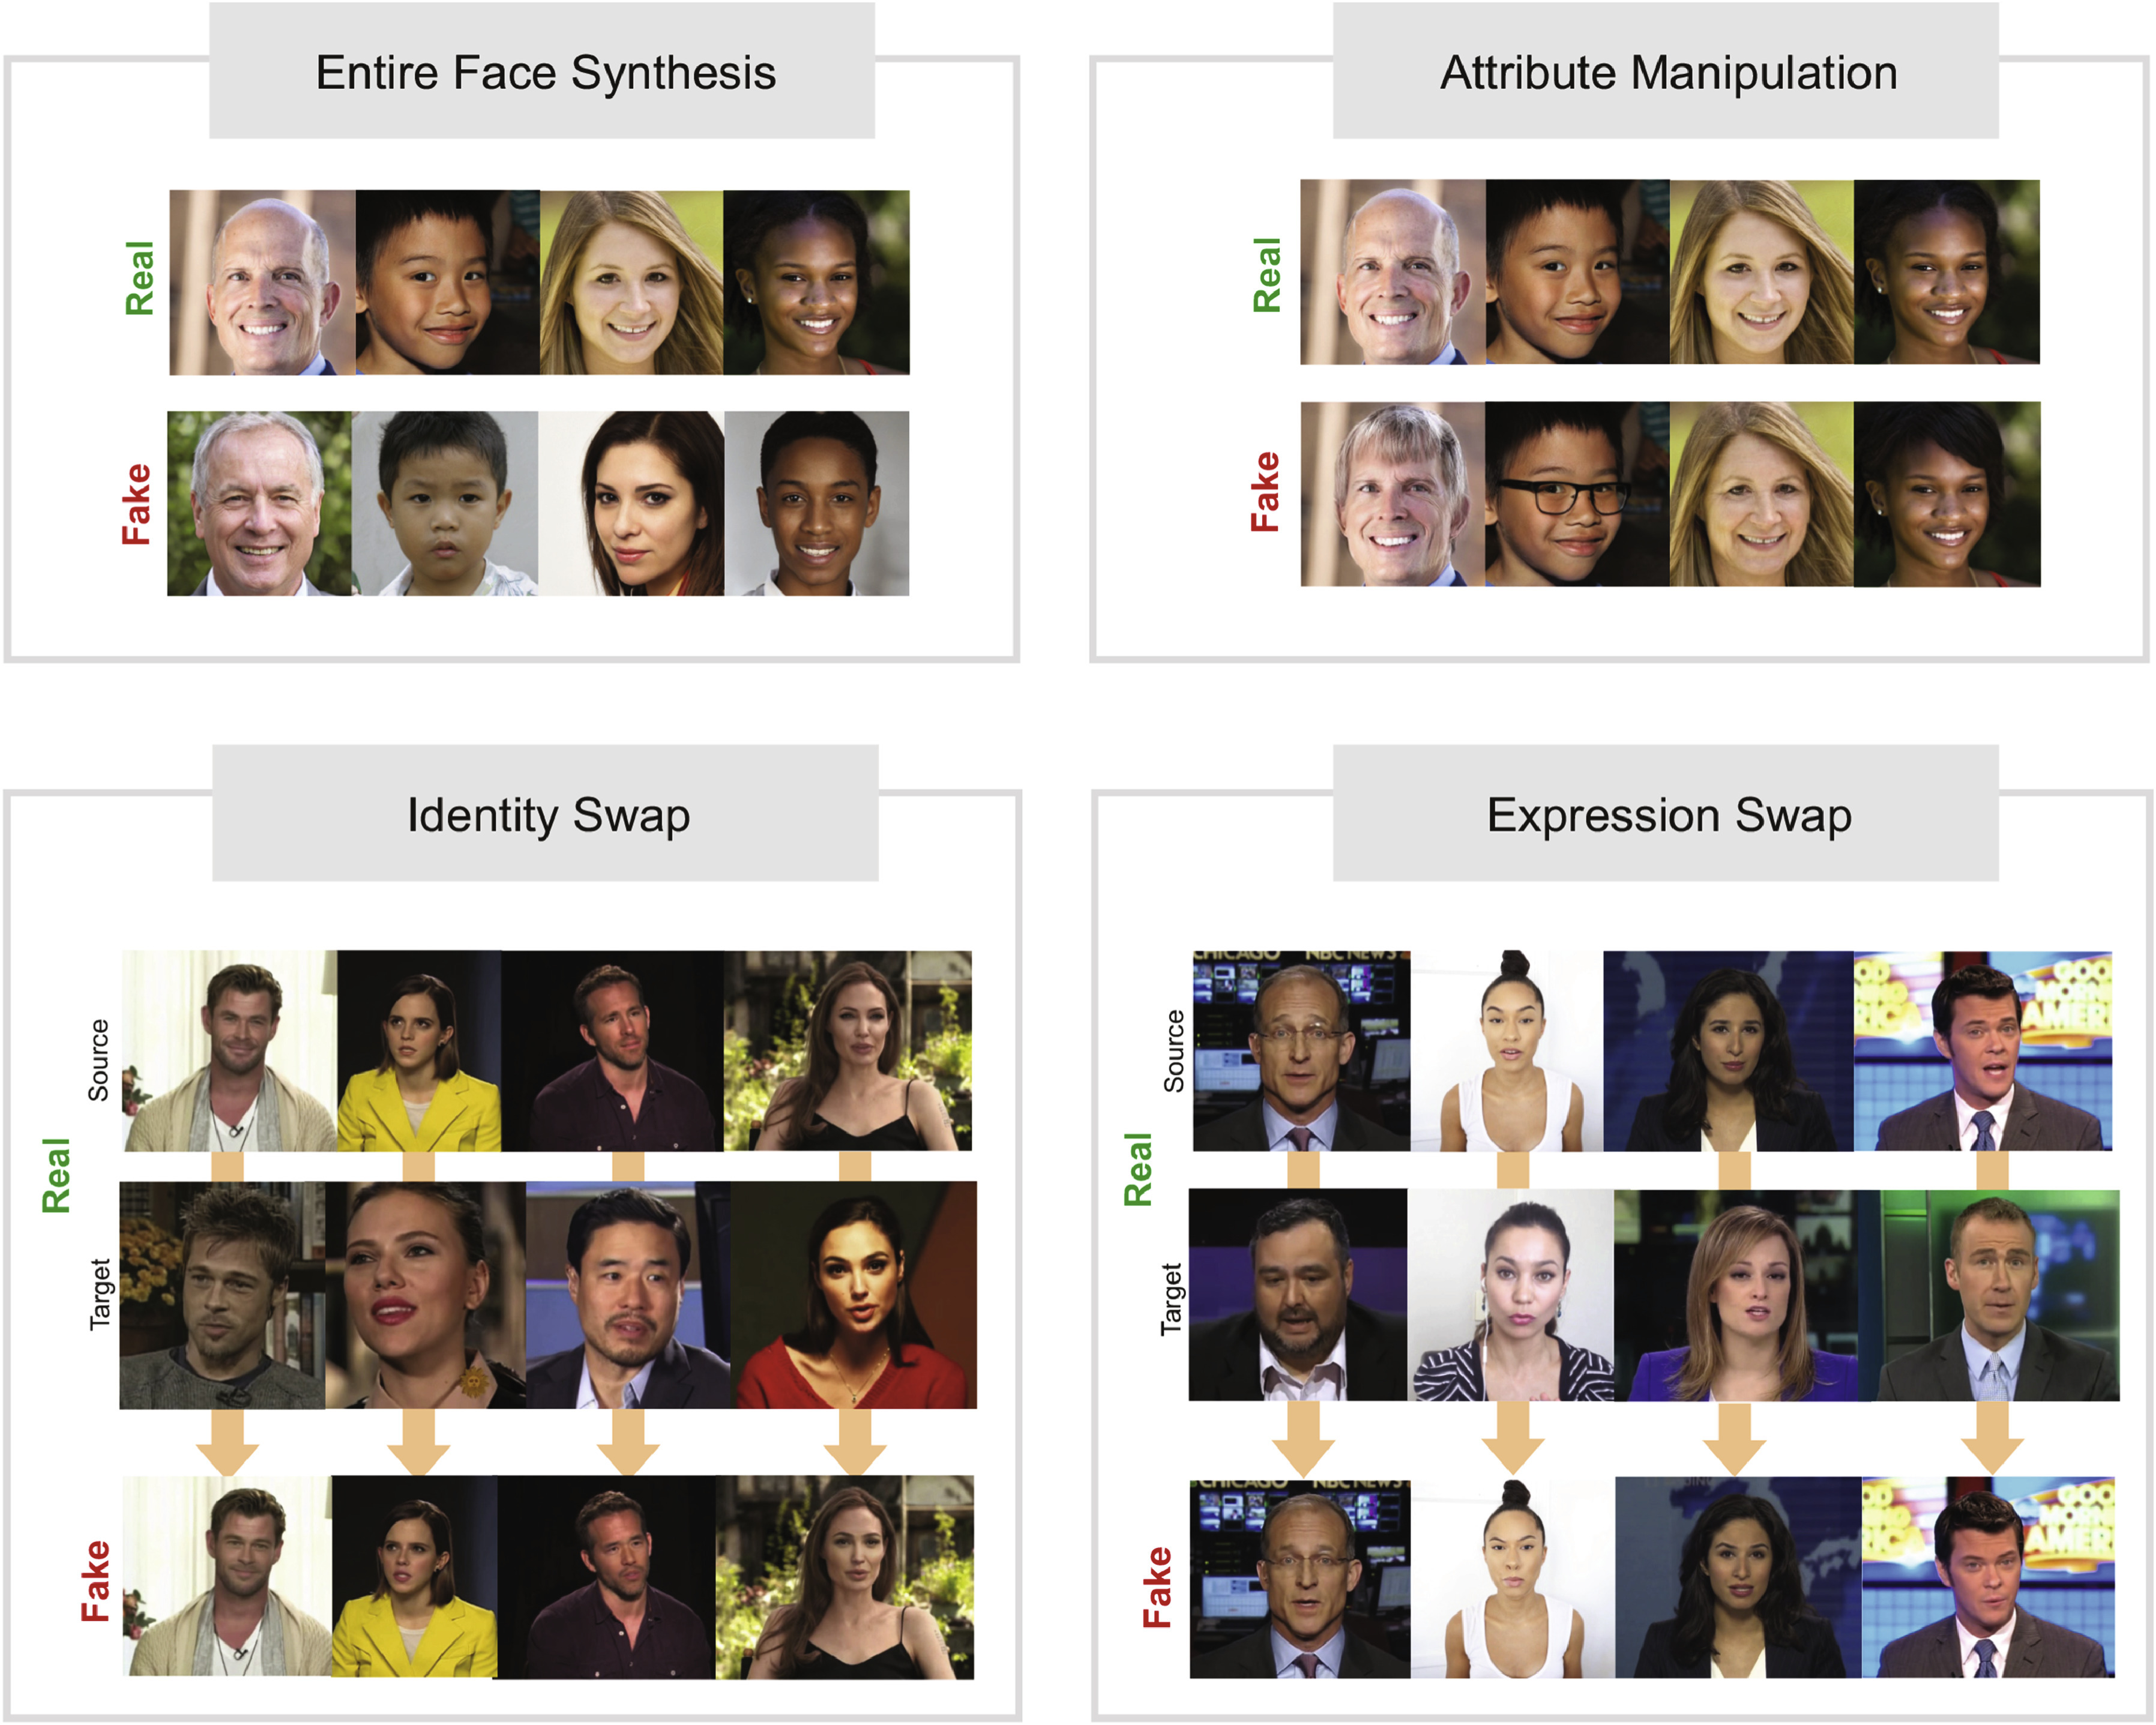
\includegraphics[width=1\linewidth]{img/face manipulations.jpg}
     \caption{Esempi per ogni tipo di manipolazione di volti}
     \label{fig:facemanip}
\end{figure}
\subsection{Generation}
Per la creazione di immagini di volti sintetiche sono usate principalmente tre diverse architetture \cite{fernando2025face}: Autoencoders, GANs e Diffusion Models. Comprenderne il funzionamento è fondamentale per capire come sviluppare metodi per identificare le immagini prodotte.
\paragraph{Autoencoders} Sono architetture composte da un encoder che ha l'obbiettivo di trasformare l'input in una rappresentazione latente compatta ed un decoder, che ricostruisce l'immagine desiderata. Sono usate nell'identity swapping e l'idea è che un encoder comune apprende una rappresentazione latente condivisa, mentre decoder separati si specializzano nella ricostruzione di immagini relative ad un individuo specifico \cite{fernando2025face}
%. Così le features latenti estratte dal volto di una persona vengono fatte passare nel decoder di un'altra persona
, così da ottenere uno scambio di identità decodificato la rappresentazione compatta della persona $A$ con il decoder della persona $B$.
\paragraph{Diffusion Models} I modelli di diffusione sono modelli probabilistici il cui funzionamento si basa su due fasi: nel \textit{forward process} l'immagine viene corrotta introducendo del rumore casuale, mentre nel \textit{reverse process} il modello viene poi addestrato a ricostruire l'immagine iniziale rimuovendo il rumore.\\
Queste fasi vengono ripetute in modo iterativo e permettono di generare immagini di alta qualità riuscendo a catturare dettagli molto fini; i Diffusion Models attualmente rappresentano lo stato dell'arte in questo campo.
\subsection{}{GANs}\ref{subsec:GAN}
GAN è l'architettura proposta nel 2014 da Goodfellow et al.\cite{goodfellow2014generative} composta da due componenti principali: generatore e discriminatore. Il generatore $G$ ha il compito di produrre delle immagini realistiche partendo da un input casuale, mentre il discriminatore $D$ deve distinguere i campioni reali da quelli generati da $G$.\\
Le due reti vengono addestrate insieme competendo una contro l'altra in un \textit{minimax game} nel quale $G$ deve massimizzare la probabilità che $D$ compia un errore. Inizialmente $G$ genererà immagini rumorose e facilmente identificabili da $D$; quest'ultimo, ricevendo in input sia immagini reali che generate da $G$, fornirà in output la probabilità che un'immagine appartenga all'insieme di immagini autentiche. Il gradiente della funzione di perdita di $D$ verrà usato per aggiornare $G$, che alla fine dell'addestramento avrà imparato a generare campioni abbastanza realistici in modo da ingannare $D$.\\
Questa architettura è stato il primo salto di qualità nel campo della generazione di immagini e per anni è stata  il punto di riferimento.
\paragraph{StyleGAN}

\subsection{Detection}
%Review of Image Forensic Techniques Based on Deep Learning 
%Media forensic
\paragraph{Approcci classici}
\paragraph{Approci basati su deeplearning}



\newpage

\section{JPEG AI} \label{sec:jpegai}
La qualità e la risoluzione delle immagini  è in continua crescita, e così la loro dimensione in formato non compresso; considerando anche l'aumento del numero di immagini prodotte e visualizzate quotidianamente, si è sviluppata la necessità di trovare dei nuovi metodi di compressione, così da permettere una trasmissione e un'archiviazione più efficienti.\\
Un nuovo promettente paradigma di compressione è chiamato"\textit{Learning-based image compression}" o "\textit{Neural image compression}" e sfrutta l'apprendimento automatico, facendo leva sulle reti neurali per raggiungere livelli di compressione maggiori.
\subsection{Compressione di immagini}
\begin{quote} 
    "\textit{A picture is worth a thousand words}"
\end{quote}
La compressione dei dati è un problema importante e ampiamente studiato nell'informatica: l'obiettivo è quello di rappresentare un'informazione usando un numero ridotto di bit rispetto alla rappresentazione originale. Nel caso delle immagini questo equivale a rappresentare la stessa informazione visiva, almeno apparentemente, riducendo lo spazio di archiviazione utilizzato.\\
La compressione si divide in due approcci: lossless,  senza perdita di informazione, e lossy, ovvero con perdita di informazione.
La compressione senza perdita viene usata quando è richiesta una ricostruzione perfetta dell'immagine originale, per esempio nel caso di immagini mediche. Quella con perdita invece scarta parte dell'informazione, in particolare dei dettagli non percettibili dall'occhio umano, per raggiungere un maggior livello di compressione; è quella usata nella condivisione delle immagini sul web.
\paragraph{Compressione lossy classica}
Tradizionalmente il processo per la compressione lossy comprende i seguenti passaggi: inizialmente all'immagine viene applicata una trasformata che mappa i pixel dal dominio spaziale ad uno più efficiente; questi coefficienti vengono poi quantizzati, fase dove si ha la principale perdita di informazione. Infine si effettua una codifica dell'entropia lossless, per trasformare la sequenza di coefficienti quantizzati in un bitstream finale.\\
Il più importante e diffuso esempio di compressione lossy è JPEG \cite{jpeg}; il suo successo è dovuto al basso costo computazionale necessario per calcolare la DCT (\textit{Trasformata discreta del coseno}), che, applicata a blocchi di $8 \times 8 $ pixel, mappa i pixel dal dominio spaziale a quello della frequenza, permettendo di concentrare la maggior parte dell'informazione rilevante in pochi coefficienti. Dopo questa trasformata i coefficienti vengono quantizzati in base alla loro frequenza, usando maggiore precisione per le frequenze più basse, che contengono più informazione per l'occhio umano, e approssimando maggiormente quelle più alte. \\
In generale  le tecniche tradizionali sono state progettate "a mano" da ingegneri e ricercatori sfruttando la conoscenza della struttura probabilistica dell'informazione; questi metodi quindi usano una trasformata fissa che ha lo svantaggio di non essere abbastanza flessibile e ottimale per tutti i tipi di immagine.

\subsection*{Learned image processing}
In questo nuovo paradigma di compressione si fruttano le reti neurali: si possono trovare articoli che propongono delle tecniche di questo tipo già negli anni '90 \cite{sonehara1989image, sicuranza1990artificial}, quando però la loro implementazione non era possibile nella pratica. Recentemente, con i progressi nell'apprendimento automatico e lo sviluppo di hardware specializzato come le GPU, anche il campo del learned image compression si è evoluto.\\
La differenza con i codec tradizionali come JPEG è che in questo nuovo approccio ogni componente classica (trasformata, quantizzazione, codifica dell'entropia) è sostituita da una rete neurale, portando così alla creazione di un \textit{learned image codec}, ovvero reti neurali che apprendono trasformate \textit{non-lineari} permettendo una rappresentazione più adatta.
\paragraph{Architettura}La maggior parte delle tecniche sono basate sugli autoencoder \cite{theis2017lossy}, un tipo speciale di rete neurale in grado di imparare la mappatura tra l'input e uno spazio di una rappresentazione latente, spesso chiamato \textit{bottleneck}.\\
L'architettura che ha riscosso più successo è quella proposta da \cite{balle2018variational} che ha dato una prova dell'efficienza di questa tecnica, migliorata successivamente da \cite{minnen2018joint}.\\
Uno degli aspetti fondamentali di queste architetture è l'approccio end-to-end nel quale tutti i moduli, dall'encoder al decoder, vengono addestrati insieme con una \textit{global loss-function} permettendo un'ottimizzazione "unificata" che massimizza l'efficienza di compressione. Questo rappresenta un grosso vantaggio rispetto ai metodi tradizionali dove invece ogni componente veniva ottimizzata separatamente.\\
Si possono trovare però anche altri tipi di architettura, e come proposto in \cite{ascenso2019report}, si possono classificare in:
\begin{itemize}
    \item tipo di rete neurale utilizzata: oltre a quelli già citati, sono usate anche RNN, per elaborare l'immagine in modo sequenziale, oppure GAN, che consente una miglior qualità visiva dell'immagine ricostruita.
    \item dimensione dell'unità di codifica: alcune tecniche scelgono di elaborare l'intera immagine, altre decidono di farlo a blocchi di piexl, riducendo la complessità
    \item strategia del controllo del bit rate: alcuni usano uno stesso modello per comprimere a più bitrate, altri invece usano diversi modelli ottimizzati per un singolo livello di qualità
\end{itemize}
%per andare più nel dettaglio consultare anche sito Neuarl image compression in nutshell cap1
\subsection{Motivazioni per lo sviluppo di JPEG AI}
%TODO: leggere  "Learning based image coding", di JPEG che ha motivato sviluppo di JPEG AI
La principale motivazione dietro lo sviluppo è descritta nel seguente modo:
\begin{quote}
    "\textit{The scope of JPEG AI is to create a learning-based image coding standard that provides a single-stream, compact compressed domain representation targeting both human visualization,.., and effectiveperformance for image processing and computer vision tasks, with the goal of supporting royalty-free baseline} \cite{ascenso2023jpegAI}"
\end{quote}
L'obbiettivo può essere paragonato alla creazione di un \textit{"linguaggio comune"} che consenta una rappresentazione  efficiente sia per la visione degli umani che delle macchine. Questa scelta risulta interessante considerando che i contenuti digitali non sono più visualizzati esclusivamente dagli umani, ma ci sono molte applicazioni dove sono le macchine i destinatari principali.
La stessa rappresentazione ricca di informazione potrebbe infatti essere usata sia per task di \textit{image processing}, che \textit{computer vision}, dove l'obbiettivo è estrarre dall'immagine informazione semantica, oppure potrebbe essere ricostruita (vedi fig. \ref{fig:fig:jpeg_frw}).
\begin{figure}
    \centering
    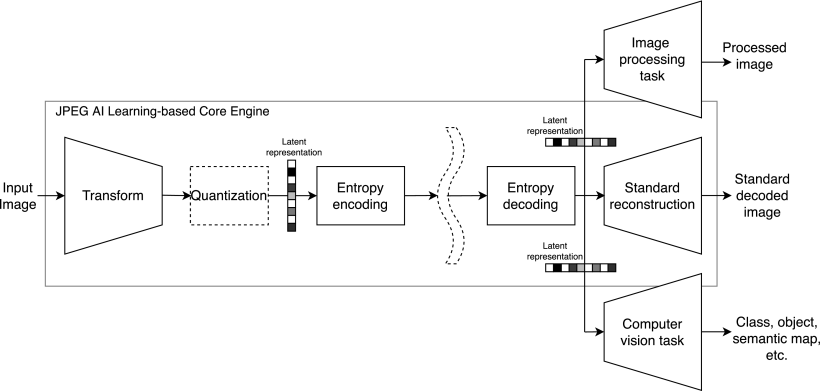
\includegraphics[width=1\linewidth]{img/JPEG AI.png}
    \caption{Framework JPEG AI}
    \label{fig:fig:jpeg_frw}
\end{figure}\\
\paragraph{Vantaggi}Un unico bitstream multitask offre due vantaggi: il primo riguarda la riduzione della complessità necessaria a svolgere task di image processing o computer vision, dato che consente di saltare completamente la parte di ricostruzione dell'immagine e di agire direttamente sulla rappresentazione latente; il secondo vantaggio riguarda l'accuratezza di alcune operazioni, infatti essendo stato progettato per contenere tutta l'informazione (anche semantica) contenuta nell'immagine originale, utilizzare direttamente la rappresentazione compatta garantirebbe un'accuratezza migliore di utilizzare l'immagine lossy ricostruita, in particolare per bitrate bassi.\\
Per ottenere questo l'encoder di JPEG AI deve generare un bitstream indipendente da tutti task, ovvero non ottimizzato per nessun compito specifico, con il requisito di mantenere sempre un alto livello di compressione.
\subsection{Architettura}\label{sec:architetturaJPEGAI}
L'architettura di JPEG AI segue le strutture tipiche di tutti i learning-based codecs,  \cite{minnen2018joint} (vedi \ref{fig:architmin}), e si può dividere in due moduli.
\begin{figure}
    \centering
    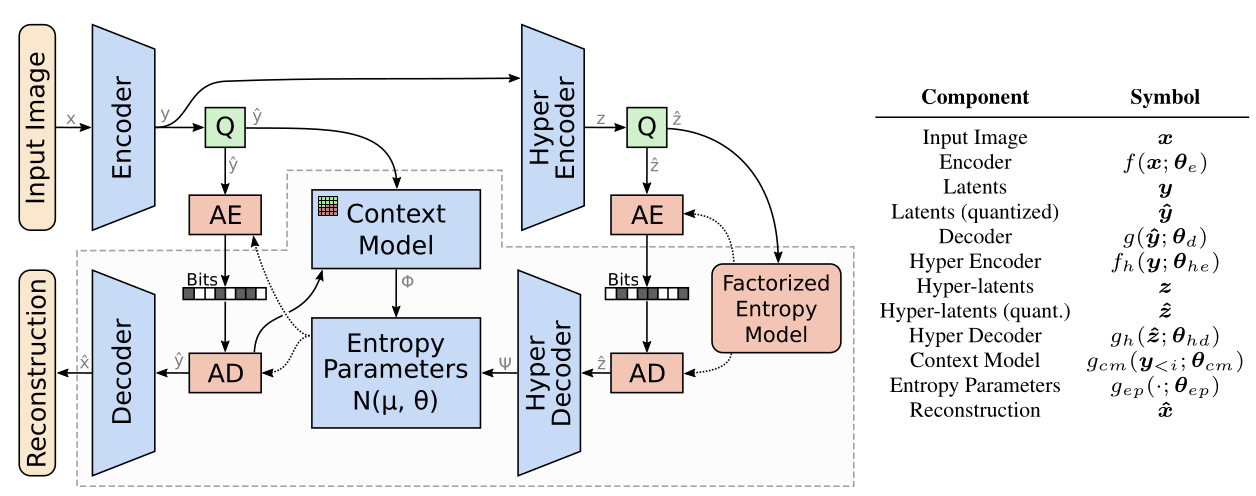
\includegraphics[width=1\linewidth]{img/architetturaJPEGAI.png}
    \caption{Architettura descritta in \cite{minnen2018joint}}
    \label{fig:architmin}
\end{figure}
Il modulo principale è quello che rappresenta l'autoencoder, composto dalla coppia \textit{encoder-decoder}.
L'encoder apprende una trasformata chiamata \textit{Analysy transform}, che mappa l'immagine $x$ in un tensore latente $y$,  mentre il decoder esegue il processo inverso, \textit{Synthesis transform}, prendendo la versione quantizzata della rappresentazione e trasformandola in immagine.\\
%TODO: menzionare del fatto che sono Non lineari??
%TODO: menzionare che spazio latente è spazio più efficiente per info visive?
Il secondo modulo corrisponde al \textit{Modello per l'entropia}; composto da \textit{Hyperprior}, e \textit{Context-model} e apprende un modello probabilistico dei latenti per svolgere in modo più efficiente la codifica dell'entropia \cite{balle2018variational}. L'\textit{Hyperprior} è composto da un \textit{hyper-encoder}, che estrae da $y$ delle \textit{side-information}  $z$ che vengono quantizzate ${(\hat{z})}$ ed  incluse nel bitstream, e un \textit{hyper-decoder}, che prendendo $z$ aiuta a predire la distribuzione dei latenti. Il \textit{Context model} invece usa i latenti per stimare l'entropia di $\hat{y}_i$ usando gli elemeni già codificati $\hat{y}_{<i}$.\\
Alcuni approfondimenti sono stati fatti nella sezione \ref{sec:vm}
\\
La pipeline di compressione è descritta nei seguenti paragrafi
\paragraph{Fase di Encoding}
Il processo di encoding di un'immagine si può osservare in \ref{fig:encodingJPEGAI}: inizialmente l'analysis transform, una rete neurale composta da layer non lineari, trasforma l'immagine in un tensore latente $y$; questo viene elaborato dall'hyper-encoder che estrae da $y$ il tensore $z$, poi viene arrotondato ($\hat{z}$) e compresso nell'ultima parte del bitstream. 
Per la codifica entropica di $y$  viene usato un hyper-scale decoder, che riceve $\hat{z}$,  per genera le varianze necessarie per fare la codifica entropica dei residui, mentre un hyper-mean decoder per produrre una stima dell'immagine originale che viene usata nel modulo di Latent Prediction, che ha il compito di stimare $\mu_y$.
Sottraendo $\mu_y$ al latente originale $y$, vengono calcolati i residui; dopo esser stati scalati e arrotondati, sono compressi nel bitstream usando me-tANS.\\
\begin{figure}
    \centering
    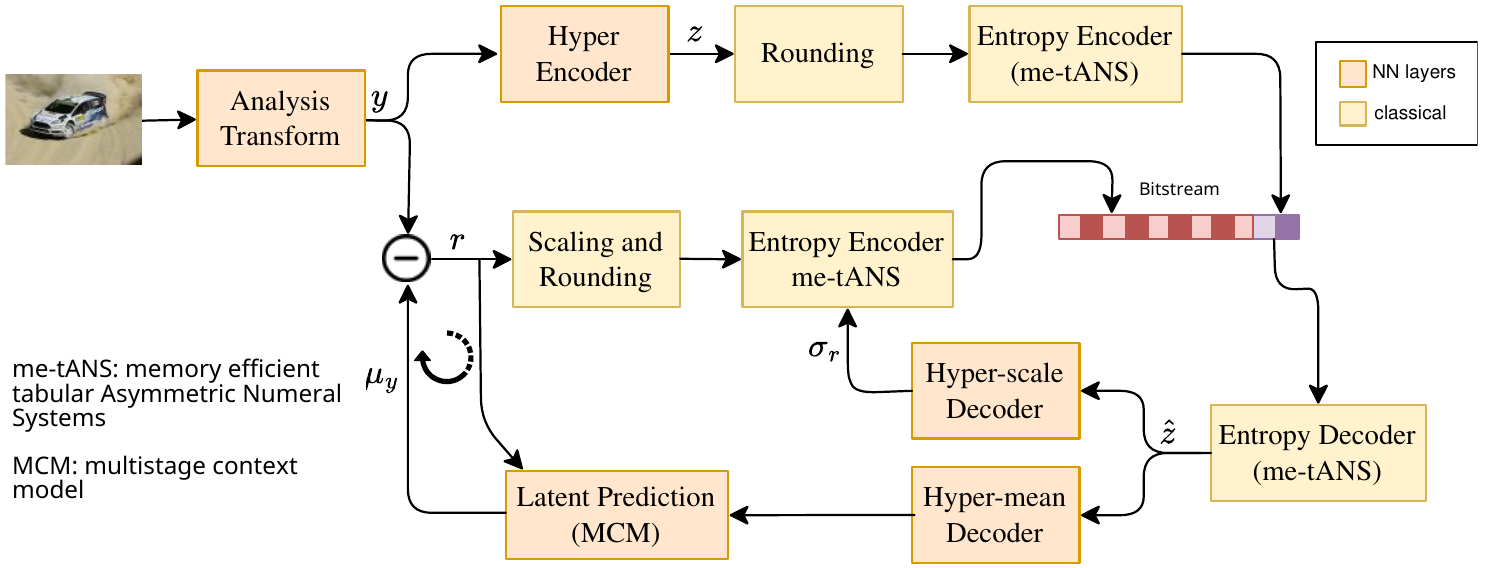
\includegraphics[width=1\linewidth]{img/encongdingJPEGAI.png}
    \caption{Schema della fase di encoding}
    \label{fig:encodingJPEGAI}
\end{figure}
\paragraph{Fase di Decoding}
Nella fase di decoding (vedi fig. \ref{fig:decodingJPEGAI}) avviene esattamente il processo inverso: inizialmente viene fatta la decodifica delle informazioni ausiliari $\hat{z}$ , usate per decodificare in modo più efficiente i residui, ottenndo $\hat{r}$. Attraverso un modo di latent prediciont vengono nuovamente stimati $\hat{y}$, che è ricevuta dalla synthesis transform che produce un'immagine partendo dalla rappresentazione latente ricevuta.
\begin{figure}
    \centering
    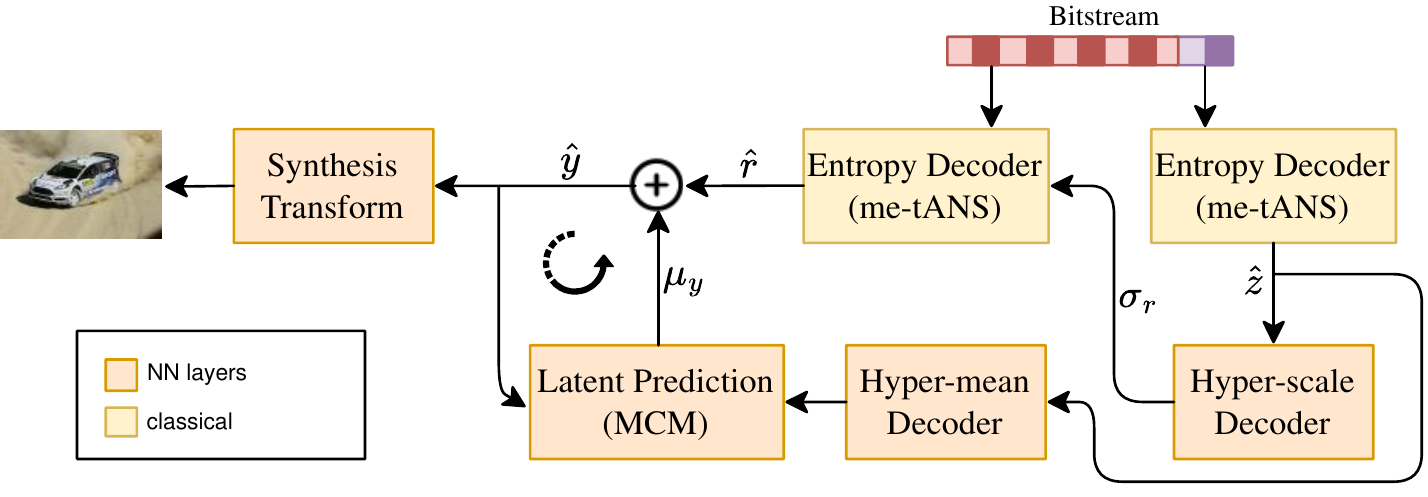
\includegraphics[width=1\linewidth]{img/decodingJPEGAI.png}
    \caption{Fase di Decoding di JPEG AI}
    \label{fig:decodingJPEGAI}
\end{figure}
\\
Si rimanda alla sez. \ref{sec:vm} per la descrizione della vera implementazione,
\paragraph{Risultati ottenuti da JPEG AI}\label{par:riep}
I primi esperimenti hanno avuto già risultati promettenti, infatti con le prime versioni delle implementazioni, JPEG AI è riuscito a raggiungere un BD-rate gain (parametro standard per la valutazione della compressione) del 28\% \cite{ascenso2023jpegAI}  rispetto a VVC Intra (lo standard attuale più efficiente) usando la configurazione più semplice "\textit{tools-off"}, ovvero usando solo gli strumenti di base per codifica e decodifica. Inoltre è stato notato anche un miglioramento rispetto al livello di qualità soggettiva a parità di bitrate \cite{ascenso2023jpegAI}, constatando l'importanza e il potenziale di questo strumento.
\section{Riepilogo}
%TODO: leva i riepiloghi
%TODO: leggere Deep Architectures for Image Compression: A Critical Review
%TODO: DIRE CHE già si vede alta compressione.
%TODO: SPIEGARE COSA CAMBIA FA ALTRI LAVORI (per esempio quello che fa stessa cosa delle facce lo fa usando bridge)
In letteratura si possono già trovare molte tecniche di Learned image compression \cite{ascenso2019report}, ma l'importanza di JPEG AI  sta nel fatto di essere diventato il primo standard ufficiale di questo tipo \cite{JPEG106thMeeting}; considerando  gli obbiettivi, i requisiti, le key task dichiarate ed i risultati ottenuti \ref{par:riep}, è possibile che questo standard verrà adottato su larga scala, rendendolo un riferimento per studi e applicazioni in futuro.\\
L'obbiettivo di questa tesi è capire se la rappresentazione latente prodotta dell'encoder di JPEG AI è sufficiente a task di fake detection, testando così le dichiarazioni fatte per la creazione di questo strumento.

